\documentclass{article}
\usepackage{graphicx, color}
\usepackage{amsmath, amssymb}

\setlength{\textwidth}{6.5in}
\setlength{\textheight}{8.5in}
\setlength{\oddsidemargin}{0in}
\setlength{\evensidemargin}{0in}
\setlength{\parskip}{2ex}
\setlength{\parindent}{0in}



\begin{document}
%To display answers, replace "white" with "red".
\newcommand{\answer}[1]{\color{white}#1}

\pagestyle{myheadings}\markright{
CU Boulder \hspace{0.5in} MATH 2510 - Introduction to Statistics }

\begin{center}
\textbf{\underbar{In-class Worksheet 23}}
\end{center}

\begin{enumerate}

%Section 9.1 #18
\item Do larger universities tend to have more property crime?  Let $x$ be a variable that represents student enrollment (in thousands) on a campus, and let $y$ be a variables that represents the number of burglaries per year on the campus.  A random sample of $n=8$ universities in California gave the following information about enrollments and annual burglary incidents (Reference: {\em Crime in the United States}, Federal Bureau of Investigation). 

\begin{center}
\begin{tabular}{c|llllllll}
\hline
$x$ & 12.5 & 30.0 & 24.5 & 14.3 & 7.5 & 27.7 & 16.2 & 20.1 \\
\hline
$y$ & 26 & 73 & 39 & 23 & 15 & 30 & 15 & 25 \\
\hline
\end{tabular}
\end{center}

	\begin{enumerate}
	\item Make a scatter diagram and then draw a line that seems to `best-fit' your data. 
	%Use WS31_1Ans.jpg for answer key
	
	\begin{center}
	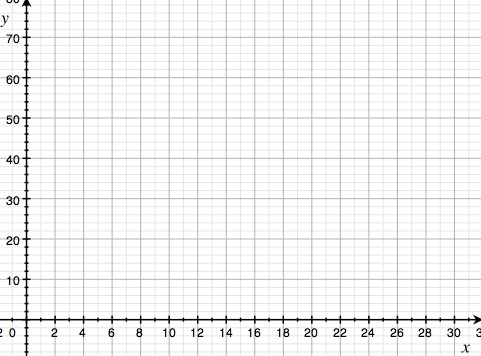
\includegraphics[scale=0.7]{WS23_1Grid.jpg} 
	%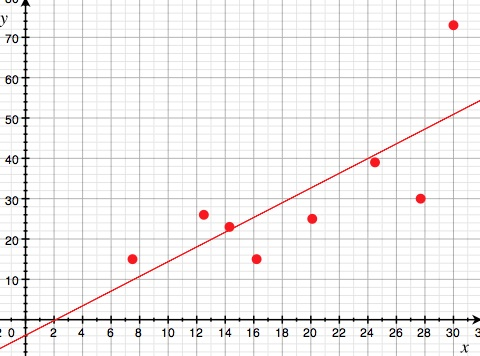
\includegraphics[scale=0.7]{WS23_1Ans.jpg}
	\end{center}
	
	\item Is the correlation between $x$ and $y$ negative or positive?  Explain.
	
	{\answer  Because the line slopes upward, the correlation is positive.} 
	
	\vfill
	
	\item Compute the correlation coefficient $r$.  Does this indicate that there is a low, moderate, or high linear correlation?
	
	{\answer With $L_1 = x$ and $L_2 = y$, \texttt{LinReg(a+bx)\{$L_1$,$L_2$\}}  yields $r=0.764841721$ which implies a moderate linear correlation.} 
	
	\vfill
	
	\end{enumerate}

\pagebreak

%Section 9.1 #10
\item Over the past 30 years in the United States, there has been a strong negative correlation between the number of infant deaths at birth and the number of people over the age of 65.  Explain what this means, then explain if
it is likely that one is causing the other?  If not, what other explanation might there be?

{\answer A strong negative correlation between these variables implies that as the number of people over the age of 65 has increased, the number of infant deaths at births has decreased.  It is unlikely that the fact that people are living longer is causing a decrease in infant mortality.  More likely, there is some lurking variable like better health care and treatments.
}
\vfill

%Section 9.2 #18
\item Did you know that it is possible to use the cricket as a thermometer?  Crickets tend to chirp more frequently as temperatures increase.  This phenomenon was studied in detail by George W.\ Pierce, a physics professor at Harvard.  In the following data, $x$ is a random variable representing chirps per second and $y$ is a random variable representing temperature ($^\circ$F). 

\begin{center}
\begin{tabular}{c||ccccccccccccccc}
\hline
$x$ & 20.0 & 16.0 & 19.8 & 18.4 & 17.1 & 15.5 & 14.7 & 17.1 & 15.4 & 16. 2 & 15.0 & 17.2 & 16.0 & 17.0 & 14.4 \\
\hline
$y$ & 88.6 & 71.6 & 93.3 & 84.3 & 80.6 & 75.2 & 69.7 & 82.0 & 69.4 & 83.3 & 79.6 & 82.6 & 80.6 & 83.5 & 76.3 \\ 
\hline
\end{tabular}
\end{center}

	\begin{enumerate}
	\item Determine the value of the sample correlation coefficient $r$.  Does $r$ indicate a weak or strong linear correlation? 
	
	{\answer With $L_1 = x$ and $L_2 = y$, \texttt{LinReg(a+bx)\{$L_1, L_2$\}} yields, $r = 0.8351437868$ which implies a moderate correlation.
	} 
	
	\vfill
	
	\item Find the equation of the least-squares line $\hat{y} = a +bx$. 
	
	{\answer \texttt{LinReg(a+bx)\{$L_1, L_2$\}} yields $\hat{y} = 25.2323131 + 3.291094089x$.
	} 
	
	\vfill
	
	\item What is the predicted temperature when $x =19$ chirps per second? 
	
	{\answer Plugging in $x=19$, $\hat{y} =  25.2323131 + 3.291094089(19) = 87.76310079$. 
	So, the predicted temperature is $87.8^\circ$F.
	} 
	\vfill
	
	\end{enumerate}

\vfill
\pagebreak

%Section 9.2 #10
\item Data for this problem are based on information from {\em STATS Basketball Scoreboard}.  It is thought that basketball teams that make too many fouls in a game tend to lose the game even if they otherwise play well.  Let $x$ be the number of fouls that were more (i.e., over and above) than the number of fouls that the opposing team made.  Let $y$ be the percentage of times the team with the larger number of fouls won the game. 

\begin{center}
\begin{tabular}{c|rrrr}
\hline
$x$ & 0 & 2 & 5 & 6 \\
\hline
$y$ & 50 & 45 & 33 & 26 \\
\hline
\end{tabular}
\end{center}

	\begin{enumerate}
	\item Is the correlation positive or negative? 
	
	{\answer There is a negative correlation between $x$ and $y$.  As the number of fouls above and beyond the opposing team goes up, the winning percentage goes down.
	} 
	
	\vfill
	
	\item How strong is the linear correlation between these two variables? 
	
	{\answer With $L_1=x$ and $L_2=y$, \texttt{LinReg(a+bx)\{$L_1, L_2$\}} yields, $r= -0.987594662$.  This value of $r$ indicates a fairly strong linear correlation.
	} 
	
	\vfill
	
	\item Find the equation of the least-squares line $\hat{y} = a +bx$. 
	
	{\answer \texttt{LinReg(a+bx)\{$L_1, L_2$\}} yields $\hat{y} = 51.28571429 - 3.934065934x$.
	} 

	\vfill
	
	\item If a team has $x=4$ fouls over and above the opposing team, what does the least-squares equation forecast for $y$? 
	
	{\answer Plugging in $x=4$, $\hat{y} = 51.28571429 - 3.934065934(4) = 35.54945055$.  \\
	So, if a team had 4 fouls above and beyond the opposing team, the percentage of times they win is 35.55\%.
	} 
	
	\vfill
	
	\item Find the value of $r^2$.  What percentage of the variation in $y$ can be explained by the corresponding variation in $x$ and the least-squares line?  What percentage is unexplained? 
	
	{\answer \texttt{LinReg(a+bx)\{$L_1, L_2$\}} yields $r^2 = 0.9753432163$.  This implies that 97.5\% of the variation of $y$ is explained by the variation in $x$ (and the least-squares line) and the other 2.5\% is unexplained.
	} 

    \vfill
    
	\end{enumerate}

\newpage

\item As noted in the reading, the least-squares line developed with $x$ as the explanatory variable and $y$ as the response variable can only be used to predict $y$ values from specified $x$ values.  The equation for predicting $x$ values from specified $y$ values cannot be derived from the least-squares line predicting $y$ simply by solving the equation for $x$. 

In this exercise, we will take the same set of data and switch the roles of $x$ and $y$ to verify that the result is different than using algebra to solve the $y$ equation for $x$.

	\begin{enumerate}
	%
	\item Find the least-squares line of best fit for the following $(x, y)$ pairs.
	
	\begin{center}
	\begin{tabular}{c||ccccc}
	$x$ & 3 & 5 & 7 & 4 & 6 \\
	\hline
	$y$ & 5 & 8 & 13 & 8 & 11 \\
	\end{tabular} 
	\end{center}
	
	{\answer With $L_1 = x$ and $L_2= y$, \texttt{LinReg(a+bx) $L_1$, $L_2$} yields, $a = -0.5$ and $b = 1.9$.  So, the least-squares line of best fit for these pairs is $y = \frac{19}{10}x - \frac{1}{2}$. } 
	
	\vfill
	
	\item Solve this least squares line for $x$ and then swap $x$ and $y$.
	{\answer 
	\begin{align*} y &= \frac{19}{10}x - \frac{1}{2} \\ 
	y + \frac{1}{2} & = \frac{19}{10}x \\ 
	\frac{10}{19}y + \frac{5}{19} & = x
	\end{align*}
	
	After we swap $x$ and $y$, we get the linear equation $$y = \frac{10}{19} + \frac{5}{19}.$$
	}
	
	\vfill
	
	\item To compare, find the least-squares line of best for the swapped $(x, y)$ pairs.
	
	\begin{center}
	\begin{tabular}{c||ccccc}
	$x$ & 5 & 8 & 13 & 8 & 11 \\
	\hline
	$y$ & 3 & 5 & 7 & 4 & 6 
	\end{tabular} 
	\end{center}
	
	{\answer With $L_2 = x$ and $L_1= y$, \texttt{LinReg(a+bx) $L_2$, $L_1$} yields, $a = 0.5$ and $b = 0.5$.  So, the least-squares line of best fit for these pairs is $y = \frac{1}{2}x + \frac{1}{2}$. } 
    
    \vfill
    
	\item Do the equations from part (b) and part (c) look equivalent? 
	
	{\answer The equations do no look equivalent.  The slope for the algebraically solved line is $\frac{10}{19}$, whereas the slope for the least-squares line of best fit found in (c) is $\frac{1}{2}$.  The constant terms are quite different $\frac{5}{19}$ versus $\frac{1}{2}$.} 
	
	\vfill
	%
	\end{enumerate}
	
\end{enumerate}

\end{document}


%%%%%%%%%%%%%%%%%Questions not used%%%%%%%%%%%%%%%%%%%%%%%%%%%

\item Again, we will consider the set of data from the California universities. In this problem, you are to compare two different suggested `best-fit' lines and try to determine which one is the {\em better} fit.  The two lines to compare are

\hspace{2cm} Line 1 : $y = 1.85x -4$ \hspace{2cm} and \hspace{2cm} Line 2 : $y=1.75x -4$

To do this, fill in the following table for each line as follows: \\
(HINT: You can make the \texttt{LISTS} in your calculator do much of this work for you.)
	\begin{enumerate}
	\item First, determine the value of $\hat{y}$ using the equation of the line.
	\item Next, we need to determine how far off these $\hat y$ values are from our actual sample data $y$ in each case.  That is, how {\em wrong} are we from the actual data?  (The idea is that the `best-fit' will have the smallest cumulative error.)  Put these values in the column labeled $y - \hat y$.
	\item As you will notice, some of those values are negative ($\hat y >y$) and some are positive ($\hat y < y$).  To avoid these errors canceling each other out, we will square each of them.  Put these values in the column labeled $(y-\hat y)^2$.
	\item To complete the comparison, find the sum of each $(y-\hat y)^2$ column.  Whichever line has the smaller sum is a {\em better} fit (by the least-squares criterion). \\ 
	So, which line appears to be the better fit according to this criterion?
	\end{enumerate}

\begin{tabular}{c|c||c|c|c||c|c|c|}
$x$ & $y$ & $\hat y = 1.85x-4$ & $y-\hat y$ & $(y-\hat y)^2$ &  $\hat y = 1.75x-4$ & $y-\hat y$ & $(y-\hat y)^2$ \\
\hline
&&&&&&& \\
12.5 & 26 & {\answer{19.125}} & {\answer{6.875}} & {\answer{47.266}} & {\answer{17.875}} & {\answer{8.125}} & {\answer{66.016}} \\
& & & & & & & \\
30 & 73 & {\answer{51.5}} & {\answer{21.5}} & {\answer{462.25}} & {\answer{48.5}} & {\answer{24.5}} & {\answer{600.25}} \\
& & & & & & & \\
24.5 & 39 & {\answer{41.325}} & {\answer{-2.325}} & {\answer{5.4056}} & {\answer{38.875}} & {\answer{0.125}} & {\answer{0.01563}} \\
& & & & & & & \\
14.3 & 23 & {\answer{22.455}} & {\answer{0.545}} & {\answer{0.29703}} & {\answer{21.025}} & {\answer{1.975}} & {\answer{3.9006}} \\
& & & & & & & \\
7.5 & 15 & {\answer{9.875}} & {\answer{5.125}} & {\answer{26.266}} & {\answer{9.125}} & {\answer{5.875}} & {\answer{34.516}} \\
& & & & & & & \\
27.7 & 30 & {\answer{47.245}} & {\answer{-17.25}} & {\answer{297.39}} & {\answer{44.475}} & {\answer{-14.48}} & {\answer{209.53}} \\
& & & & & & & \\
16.2 & 15 & {\answer{25.97}} & {\answer{-10.97}} & {\answer{120.34}} & {\answer{24.35}} & {\answer{-9.35}} & {\answer{87.423}} \\
& & & & & & & \\
20.1 & 25 & {\answer{33.185}} & {\answer{-8.185}} & {\answer{66.994}} & {\answer{31.175}} & {\answer{-6.175}}  & {\answer{38.131}} \\
& & & & & & & \\
\hline
Sum & & & & {\answer{1026.2095}} & & & {\answer{1039.77625 }} \\
\end{tabular}
 \\
 
 {\answer Because the sum of the squares for Line 1 is smaller than the sum for Line 2, we consider Line 1 a better fit.}
 